% This file allows to produce either a separate PDF/PNG image
% See standalone documentation to understand underlying magic

\documentclass[tikz,convert={density=150,size=600,outext=.png}]{standalone}
\usetikzlibrary{shapes, calc, arrows, fit, positioning, decorations, patterns, decorations.pathreplacing, chains, snakes}
\input{../setup-web-fonts}
\input{../setup-packages}
\graphicspath{{../pictures/}} % path to pictures, trailing slash is mandatory.

% The actual drawing follows
\begin{document}
    \begin{tikzpicture}     
        \node[inner sep=0pt] (rack-system) {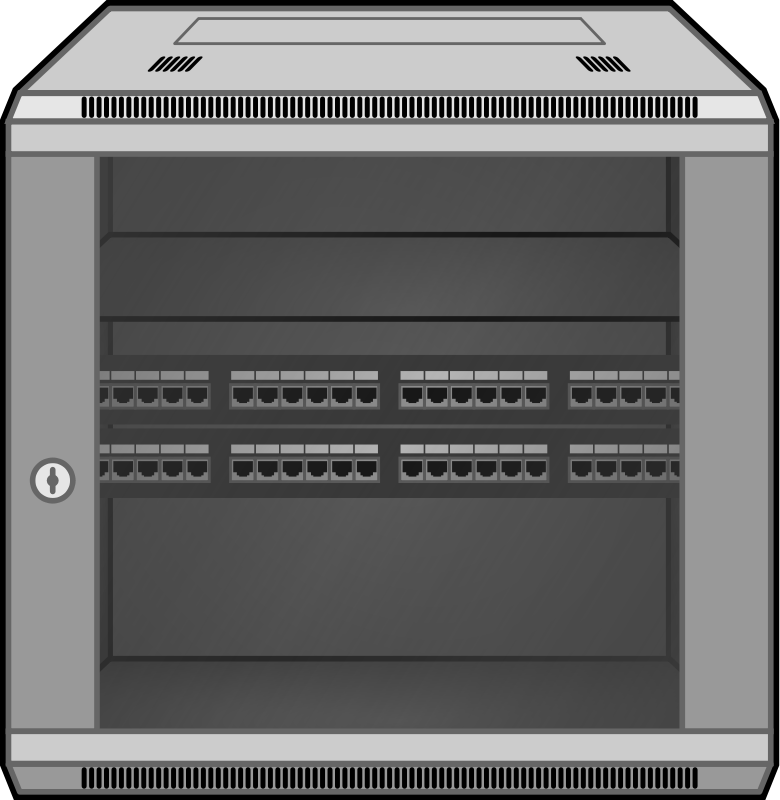
\includegraphics[width=2.5cm]{rack-system.png}};
        \node[above=0cm of rack-system, font=\footnotesize] {Модель};
        \node[cloud, draw, aspect=1.5, text width=3.2cm] at (rack-system) (cloud) {};
        
        \node[right=2cm of rack-system, yshift=-1cm] (laptop) {
\includegraphics[width=2.2cm]{laptop.png}};
        \node[color=white, anchor=base, font=\footnotesize, yshift=0.2cm] at (laptop) {\textbf{Симулятор}};
        
        \path[] (cloud) -- (laptop) node[draw, pos=0.6, sloped, single arrow, text width=0.4cm] {};
    \end{tikzpicture}
\end{document}
